\subsubsection{Visualizar Empleados}
En la siguiente figura \ref{fig:Diagrama de Secuencia - Visualizar Agenda} se muestra el diagrama de secuencia que corresponde a la visualización de cada uno de los registros de los empleados que existen dentro de la base de datos, existen dos posibilidades dentro de esta actividad:
\begin{itemize}
	\item \textbf{Si existen registros:} Al momento de que el administrador entra a esta parte del sistema, al existir registros de empleados, se muestra toda la información en una tabla y/o lista para su posterior gestión.  
	\item \textbf{No existen registros:} No hay empleados registrados, se muestra una tabla y/o lista vacía en pantalla.
\end{itemize}
\begin{figure}[!h]
	\centering
	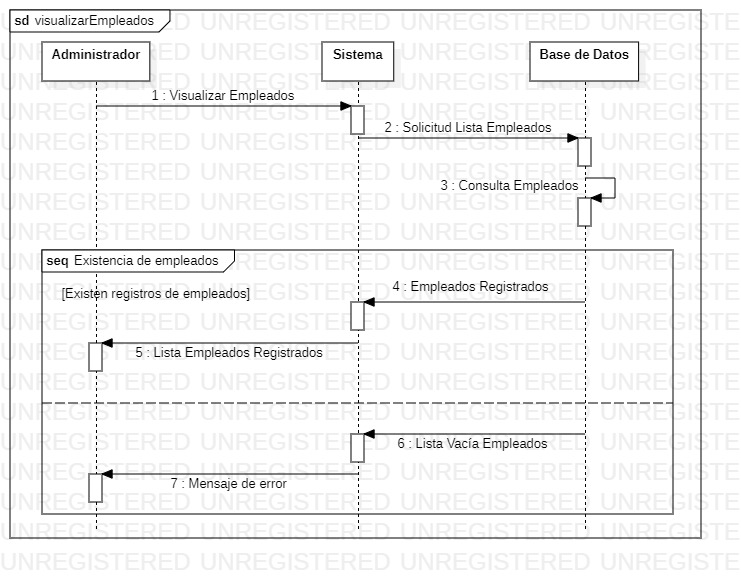
\includegraphics[width=0.8\textwidth]{./diseno/vprocesos/imagenes/visualizarEmpleados}
	\caption{Diagrama de Secuencia - Visualizar Empleados}
	\label{fig:Diagrama de Secuencia - Visualizar Empleados}
\end{figure}